\documentclass[tikz]{standalone}

\begin{document}
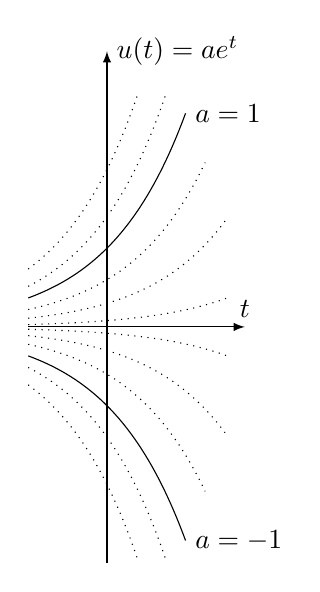
\begin{tikzpicture}
  \draw[-latex] (-1,0) -- (1.75,0) node[above] {\(t\)};
  \draw[-latex] (0,-3) -- (0,3.5) node[right] {\(u(t) = a e^t\)};
                    %
  \draw[domain=-1:1,variable=\t,samples=200]
  plot({\t}, {exp(\t)}) node [right] {\(a=1\)};
                    % 
  \draw[domain=-1:1,variable=\t,samples=200]
  plot({\t}, {-exp(\t)}) node [right] {\(a=-1\)};
                    %
  \foreach \a in {-2, 2}
  {
    \draw[domain=-1:0.4,variable=\t,samples=200,dotted]
    plot({\t}, {\a*exp(\t)});
  }
                    %
  \foreach \a in {-1.4, 1.4}
  {
    \draw[domain=-1:0.75,variable=\t,samples=200,dotted]
    plot({\t}, {\a*exp(\t)});
  }
                    %
  \foreach \a in {-0.6, 0.6}
  {
    \draw[domain=-1:1.25,variable=\t,samples=200,dotted]
    plot({\t}, {\a*exp(\t)});
  }
                    %
  \foreach \a in {-0.3, 0.3}
  {
    \draw[domain=-1:1.5,variable=\t,samples=200,dotted]
    plot({\t}, {\a*exp(\t)});
  }
                    %
  \foreach \a in {-0.08, 0.08}
  {
    \draw[domain=-1:1.55,variable=\t,samples=200,dotted]
    plot({\t}, {\a*exp(\t)});
  }
\end{tikzpicture}
\end{document}
